\documentclass[hide notes,intlimits]{beamer}

\mode<presentation>
{
  \usetheme[headline,footline]{UAFshade}
  \setbeamercovered{transparent}
}

% load packages
\usepackage[english]{babel}
\usepackage[latin1]{inputenc}
\usepackage[T1]{fontenc}
\usepackage{lmodern}
\usepackage{multimedia}
%\usepackage{hyperref}

% Some useful commands (from ELB)
\newcommand{\bD}{\mathbf{D}}
\newcommand{\bbf}{\mathbf{f}}
\newcommand{\bF}{\mathbf{F}}
\newcommand{\bg}{\mathbf{g}}
\newcommand{\bn}{\mathbf{n}}
\newcommand{\bq}{\mathbf{q}}
\newcommand{\bT}{\mathbf{T}}
\newcommand{\bu}{\mathbf{u}}
\newcommand{\bU}{\mathbf{U}}
\newcommand{\bv}{\mathbf{v}}

\newcommand{\ddx}[1]{\ensuremath{\frac{\partial #1}{\partial x}}}
\newcommand{\ddy}[1]{\ensuremath{\frac{\partial #1}{\partial y}}}
\newcommand{\ddz}[1]{\ensuremath{\frac{\partial #1}{\partial z}}}
\newcommand{\ddt}[1]{\ensuremath{\frac{\partial #1}{\partial t}}}

\newcommand{\DDt}[1]{\ensuremath{\frac{d #1}{d t}}}

\newcommand{\Div}{\nabla\cdot}
\newcommand{\eps}{\epsilon}
\newcommand{\grad}{\nabla}
\newcommand{\half}{\frac{1}{2}}
\newcommand{\trace}{\operatorname{tr}}

\newcommand{\rinv}{\frac{1}{r}}
\newcommand{\ar}{r^{-1}\alpha}
\newcommand{\stress}{\ensuremath{\text{\Large$\sigma$\normalsize}}}
\newcommand{\devstress}{\ensuremath{\text{\Large$\tau$\normalsize}}}

% Some useful commands (from MPL)
\newcommand{\s}[1]{\ensuremath{\,\text{#1}}}
\newcommand{\unit}[1]{\ensuremath{\,\text{#1}}}




% title page
\title[Glacier Dynamics] % (optional, use only with long paper titles)
{Dynamics of Glaciers}


\author[Aschwanden] % (optional, use only with lots of authors)
{Andy Aschwanden}
% - Give the names in the same order as the appear in the paper.
% - Use the \inst{?} command only if the authors have different
%   affiliation.

\institute[ARSC] % (optional, but mostly needed)
{
  %
  Arctic Region Supercomputing Center\\
  University of Alaska Fairbanks, USA
}
% - Use the \inst command only if there are several affiliations.
% - Keep it simple, no one is interested in your street address.

\date{McCarthy Summer School, June 2012}

\titlegraphic{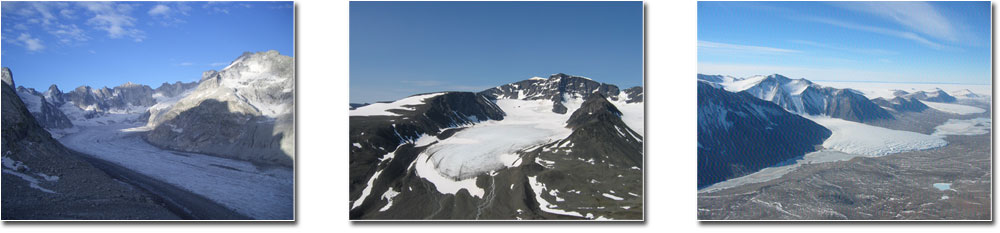
\includegraphics[width=10cm]{figures/glaciers3}}


\subject{Glaciers}

\begin{document}

\AtBeginSection[]
{
  \begin{frame}<handout:0>
    \frametitle{Outline}
    \tableofcontents[sectionstyle=show/shaded,subsectionstyle=hide]
  \end{frame}
}


% insert titlepage
\begin{frame}
  \titlepage
\end{frame}



\section{Introduction}
\label{sec:introduction}

\begin{frame}
  \frametitle{What's covered}
  We will discuss the following points:
  \begin{itemize}
  \item Parallel sided slab
  \item Flow through a cylindrical channel
  \item Flow along a longitudinal profile
  \item Free surface flow: ``The spatial mass balance is the change of elevation with time (i.e., vertical velocity) at every point on the surface.`` \emph{Konrad et. al.} (1999)
  \item Driving stress: Why is the driving stress always $\approx 1$bar?
 \end{itemize}
\end{frame}


\begin{frame}
  \frametitle{On Notation}
  \begin{itemize}
  \item (hopefully) consistent with Continuum Mechanics (Truffer)
  \item with lots of input from \emph{Luethi \& Funk: Physics of Glaciers I} lecture at ETH
  \item notation following Greve \& Blatter: Dynamics of Ice Sheets and Ice Sheets
  \end{itemize}
  \begin{figure}
    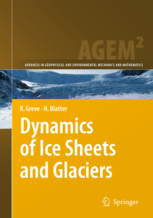
\includegraphics[scale=1.25]{figures/greveblatter_disg}
  \end{figure}
\end{frame}


\begin{frame}{Parallel Sided Slab}
  \begin{figure}
    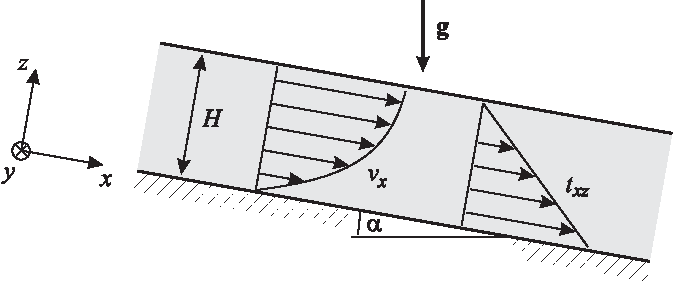
\includegraphics[width=7cm]{figures/fig_3_11}
  \end{figure}
  \begin{equation*}
    \begin{array}{ccl}
      \frac{\partial u}{\partial z}  & = &  2\,A(T,p)\,\tau^{n-1}\tau \qquad \Rightarrow \\[1em]
      u_{h} - u_{b} &  = & \int_{0}^{h} 2\,A\left(\rho\,g\,\sin{\alpha}\,z\right)^{n}\,dz =
    \end{array}
  \end{equation*}
  \\[.75em]
  We assume $u_b=0$, i.e. glacier is frozen to the bed
\end{frame}

\begin{frame}{Flow Through a Cylindrical Channel}

\end{frame}

\begin{frame}
  \frametitle{How does a glacier move?}
  \centering{
    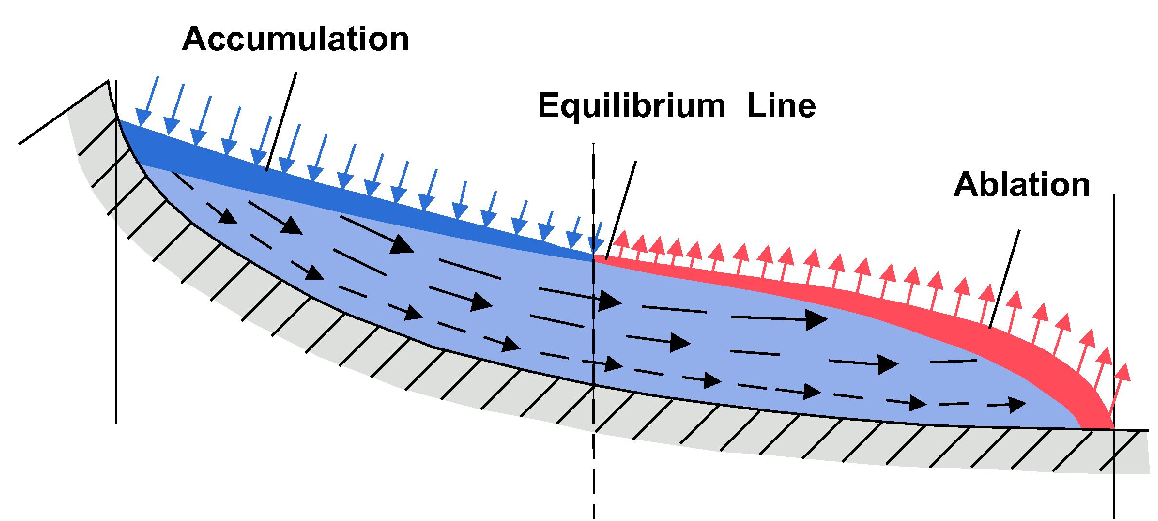
\includegraphics[width=.65\textwidth]{figures/flow_acc_abl}
  }
  \begin{block}{In a nut shell:}
    \begin{itemize}
    \item The ice can deform as a viscous fluid
    \item The ice can slide over its substrate
    \item Well-described by continuum mechanics
    \end{itemize}
  \end{block}
\end{frame}


\begin{frame}
  \frametitle{Free Surface}
  \begin{figure}
    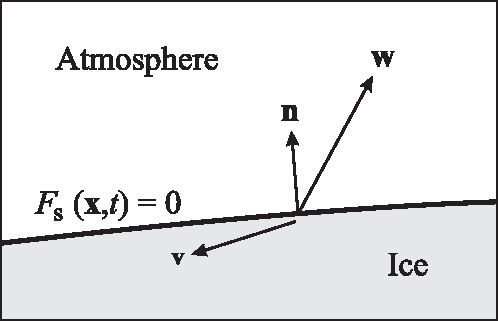
\includegraphics[width=4cm]{figures/fig_5_03}%
  \end{figure}
  \begin{itemize}
  \item on the black-board
  \item or p. 65\,--70 in the book
  \item $\mathbf{w}$ and $\mathbf{v}$ are the velocity of the free surface and the ice velocity, respectively
  \item $\mathbf{n}$ is the outward-pointing normal vector
    \begin{equation*}
      \mathbf{n} = \frac{\nabla F_{s}}{\vert \nabla F_{s} \vert}
    \end{equation*}
  \end{itemize}
\end{frame}

\begin{frame}
  \frametitle{Kinematic Boundary Condition}
  \begin{block}{Surface}
    \begin{equation}
      \frac{\partial h}{\partial t} + v_{x}\frac{\partial h}{\partial x} + v_{y}\frac{\partial h}{\partial y} - v_{z} = a_{s}
    \end{equation}
    \begin{itemize}
    \item $a_{s}$ is the \alert{accumulation-ablation} function
      \item climatic input from measurements or (melt) models
    \end{itemize}
  \end{block}
  \begin{block}{Base}
    \begin{equation}
     \frac{\partial b}{\partial t} + v_{x}\frac{\partial b}{\partial x} + v_{y}\frac{\partial b}{\partial y} - v_{z} = a_{b}
    \end{equation}
    \begin{itemize}
    \item $a_{b}$ is the \alert{basal melt rate}
      \item often $\partial b/\partial t = 0$
    \end{itemize}
  \end{block}
\end{frame}

\begin{frame}
  \frametitle{Ice-Thickness Equation}
  By combining the basal and surface kinematical equation we can obtain
  \begin{equation}
    \frac{\partial H}{\partial t} = - \nabla \cdot \mathbf{Q} + a_{s} - a_{b}
  \end{equation}
    \begin{itemize}
    \item $ a_{s}$ and $a_{b}$ are in the vertical direction
    \item the volume flux $\mathbf{Q}$ is defined as
      \begin{equation*}
        \mathbf{Q} =
        \left(
          \begin{array}{c}
            \int_{b}^{h} v_{x} \,\text{d} z \\[.25em]
          \int_{b}^{h} v_{y} \,\text{d} z
        \end{array}
      \right)
    \end{equation*}
  \item derivation on p. 70\,--\,72
  \item this is the central evolution equation in ice sheet dynamics
  \end{itemize}
\end{frame}

\end{document}
